\chapter{Листинги программы}
На листинге \ref{lst:odu} представлен листинг алгоритмов численных методов.
\begin{lstlisting}[label=lst:odu, caption=Код вычисления численных методов]
def f(self, x, y):
	"""
	Исходная функция u(x) = x^2 + u^2
	"""
	return x * x + y * y
	
def calc_euler_method(self, last_x, last_u) -> None:
	"""
	Метод Эйлера
	"""
	return last_u + self.step * self.f(last_x, last_u)
	
def calc_picard_1_method(self, x):
	"""
	Метод Пикара I порядка точности
	"""
	return pow(x, 3) / 3
	
def calc_picard_2_method(self, x):
	"""
	Метод Пикара II порядка точности
	"""
	return self.calc_picard_1_method(x) + pow(x, 7) / 63
	
def calc_picard_3_method(self, x):
	"""
	Метод Пикара III порядка точности
	"""
	return self.calc_picard_2_method(x) + 2 * pow(x, 11) / 2079 + \
	pow(x, 15) / 59535
	
def calc_picard_4_method(self, x):
	"""
	Метод Пикара IV порядка точности
	"""
	return pow(x, 31) / 109876902975 + \
	4 * pow(x, 27) / 3341878155 + \
	4 * pow(x, 23) / 99411543 + \
	2 * pow(x, 23) / 86266215 + \
	82 * pow(x, 19) / 37328445 + \
	13 * pow(x, 15) / 218295 + \
	2 * pow(x, 11) / 2079 + \
	self.calc_picard_2_method(x)
	
def calc_runge_kutt_method(self, last_x, last_u):
	"""
	Метод Рунге-Кутта
	при значении alpha = 1
	""" 
	return last_u + self.step * self.f(last_x + self.step / 2, 
	last_u + self.step / 2 * self.f(last_x, last_u))
\end{lstlisting}

\chapter{Результаты работы}
На рисунке \ref{img:methods} представлена зависимость решения уравнения от методов.
\begin{figure}[H]
	\centering{
		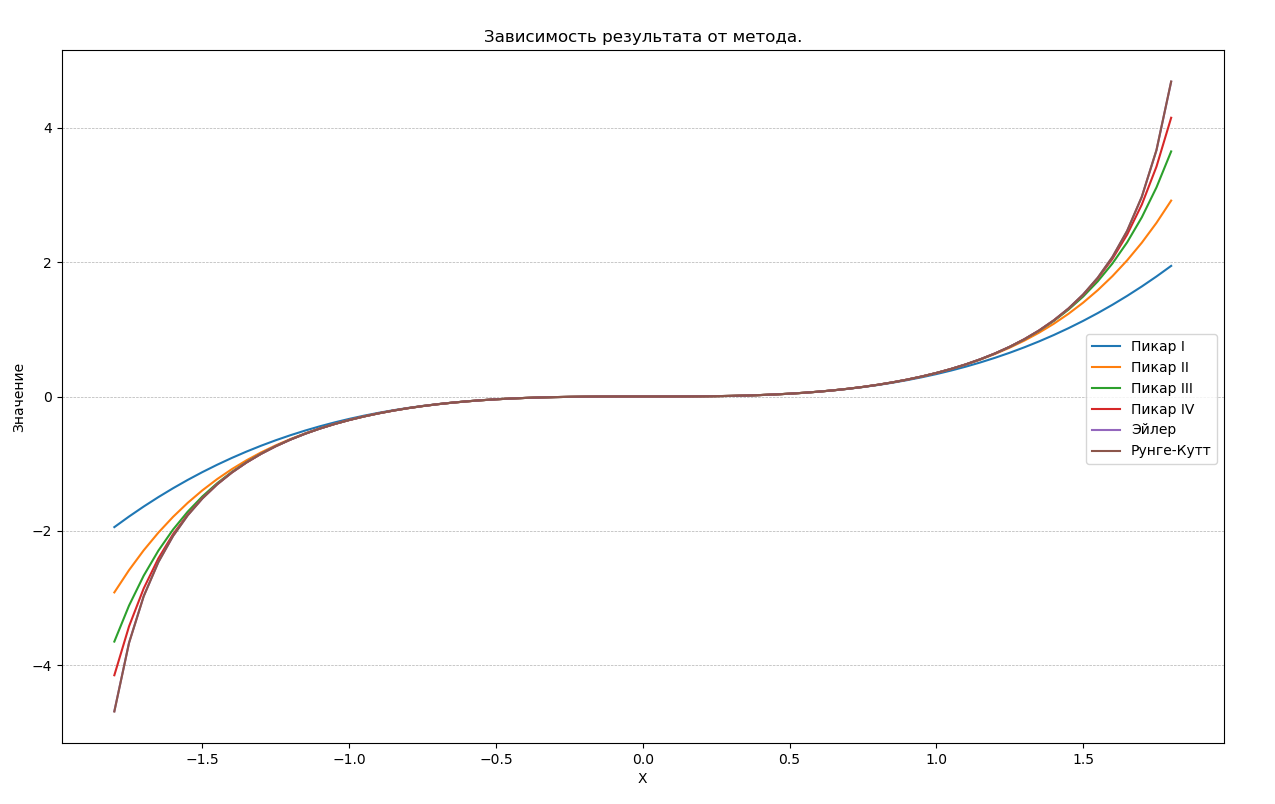
\includegraphics[scale=0.35]{images/methods}
		\caption{Зависимость решения уравнения от методов.}
		\label{img:methods}}
\end{figure} 

На рисунке \ref{img:table} представлена таблица полученных значений методов с точностью до двух знаков после запятой.
\begin{figure}[H]
	\centering{
		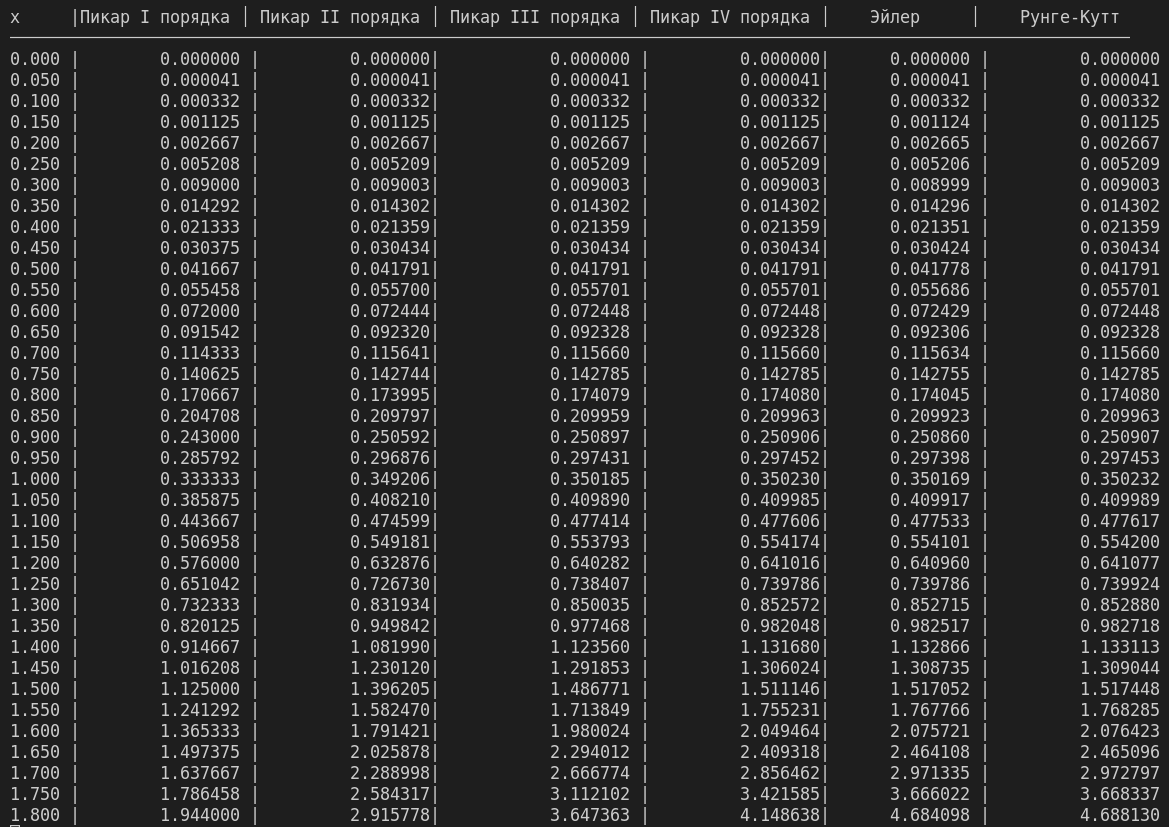
\includegraphics[scale=0.4]{images/table}
		\caption{Таблица значений.}
		\label{img:table}}
\end{figure} 

\chapter{Контрольные вопросы}
\begin{enumerate}
	\item \textbf{Укажите интервалы значений аргумента, в которых можно считать решением заданного уравнения каждое из первых 4-х приближений Пикара, т.е. для каждого приближения указать свои границы применимости. Точность результата оценивать до второй цифры после запятой.}
	
	Границы каждого из приближений определяются путем сравнивания результатов со следующим приближением с точностью до двух знаков после запятой. Если они при определенном значении аргумента отличаются, то верхняя граница не входит в интервал.
	
	Применимость метода Пикара I порядка: [0; 0.85]
	
	Применимость метода Пикара II порядка: (0.85; 1.15]
	
	Применимость метода Пикара III порядка: (1.15; 1.30]
	
	Применимость метода Пикара IV порядка: для определения верхней границы, необходимо вычислить приближение V порядка точности.
	
	\item \textbf{Пояснить, каким образом можно доказать правильность полученного результата при фиксированном значении аргумента в численных методах.}
	
	Правильность полученного значения в численных методах можно доказать следующим образом:
	
	\begin{equation}
		h \rightarrow 0; \ |y_i - u(x_i)| \rightarrow 0,
	\end{equation}

	где $u(x_i)$  -- точное значение, $y_i$ -- приближенное.
	
	\item \textbf{Каково значение решения уравнения в точке x=2, т.е. привести значение u(2).}
	
	Используя метод Рунге-Кутта II порядка ввиду его высокой точности относительно других, получаем значение u(2) $\approx$ 317.
	
	\item \textbf{Дайте оценку точки разрыва решения уравнения.}
	
	\item \textbf{Покажите, что метод Пикара сходится к точному аналитическому решению уравнения.}
\end{enumerate}


 



